\documentclass[conference]{IEEEtran}
%\IEEEoverridecommandlockouts
% The preceding line is only needed to identify funding in the first footnote. If that is unneeded, please comment it out.
%\usepackage{cite}
\usepackage{amsmath,amssymb,amsfonts}
\usepackage{algorithmic}
\usepackage{graphicx}
\usepackage{textcomp}
\def\BibTeX{{\rm B\kern-.05em{\sc i\kern-.025em b}\kern-.08em
    T\kern-.1667em\lower.7ex\hbox{E}\kern-.125emX}}
\usepackage{amsmath}
\usepackage{amssymb}
\usepackage{mathtools}

\usepackage[backend=biber]{biblatex}
\addbibresource{references.bib}

\DeclareMathOperator*{\argmin}{argmin}
\DeclareMathOperator{\E}{\mathbb{E}}
\newcommand{\norm}[1]{\left\lVert#1\right\rVert}

\renewcommand*{\bibfont}{\footnotesize}

\begin{document}

\title{Application of Stochastic Dynamic Programming to the Optimal Control of Hybrid Energy Storages in Electric Vehicles}

\author{\IEEEauthorblockN{Alok Deshpande}
\IEEEauthorblockA{University of Toronto - Energy Systems}
}

%\newenvironment{psmallmatrix}
%  {\left[\begin{smallmatrix}}
%  {\end{smallmatrix}\right]}

\maketitle

%\begin{abstract}
%This document is a model and instructions for \LaTeX.
%This and the IEEEtran.cls file define the components of your paper [title, text, heads, etc.]. *CRITICAL: Do Not Use Symbols, Special Characters, Footnotes, 
%or Math in Paper Title or Abstract.
%\end{abstract}

\section{Introduction}
Battery life is a factor that is critical to the operation of electric vehicles. Amongst its many effects on vehicle performance, it dictates the maximum distance that can be travelled on a single charging. Naturally, one would hope to maximize battery life.

In doing so, a common strategy being applied by vehicle designers is using a hybrid power supply, composed of a combination of a battery and a secondary energy storage. \cite{thounthong2009energy} The reason is that each of these storage devices is best suited for a specific energy demand (load) profile for the vehicle's operations, which may vary during the course of the trip. \cite{thounthong2009energy} By using a combination of storages, one may improve the efficiency of the energy delivery, and hence the battery life. Note that the secondary storage is usually a supercapacitor, and so will be referred to as such in this paper.

To optimally supply energy by controlling the storage devices, one can apply a technique called dynamic programming (DP). DP is well suited for optimal control in this situation because it can generate a control policy that takes into account any possible demand and can be administered at the rates at which demands arrive [HybridStorageMPC]. The novelty of this paper lies in formulating the two-storage stochastic control problem as a DP, and extending it to the timescales of electric vehicle operation via infinite horizon DP (IHDP). Because IHDP is computationally expensive to solve, the paper also reformulates it as a linear program (LP), making it amenable to fast solution by current solvers. 

This paper begins by providing the context for these two programming approaches. Upon modelling the problem in Section 3, the DP and IHDP problems are formulated in Section 4 and their issues explained. In Sections 5-6, the IHDP is re-cast as the LP, and its relative computational benefits shown. Finally, in Sections 7-8, numerical results for the vehicle application are shown to better compare the two approaches. Note that the IHDP and LP are compared both analytically and numerically.


\section{Background and Literature Review}
In order to improve battery lifetime in this vehicle energy management problem, experiments \cite{thounthong2009energy} show that it should be operated with steady output power, whereas the supercapacitor must be operated in the opposite manner \cite{thounthong2009energy}. DP is an iterative method of optimization that can be used for such optimal control. Previously\cite{thounthong2009energy}, it has been applied to determine the optimal amount of energy to charge and discharge from a battery (the control) so as to satisfy an energy demand ("load"). This paper extends upon that model by adding the supercapacitor operating in parallel.

The DP approach requires that the state (energy) and control variables be both quantized in value and discretized in time. For this application of DP, because precise control must be done with very small time steps to satisfy the fluctuating demand over a timeframe of hours, an extremely large number of iterations and fine discretization is involved.\cite{bertsekas1995dynamic} IHDP is a type of DP that allows for optimizing over these practically "infinite" number of iterations.

As will be explained in Section 4, a finite number of iterations is sufficient to approximate the solution to the IHDP.\cite{bertsekas1995dynamic} However, it still suffers from the issue of the embedded exhaustive search taking very long for the fine resolution required for the control. In Section 5, it is shown that LP can be used to determine the optimal costs to which the IHDP converges over its iterations.\cite{bertsekas1995dynamic} Moreover, \cite{4220813} shows that it is possible to subsequently obtain the optimal control "policy" by taking the dual. Given the rapidity of current LP solvers in comparison to exhaustive search, the author was motivated to follow this approach, as others have done.


\section{Model}

\subsection{Definitions}
\begin{itemize}
	\item $t$: discrete time step index
	\item $j$: storage device number (1: battery, 2: supercapacitor)
	\item $\alpha^{C}$: charging efficiency\hspace{1em}
	$\alpha^{D}$: discharging efficiency
	\item $\beta$: storage efficiency factor (constant)
	\item $T$: number of steps (DP horizon)
	\item $K$: weighting for discharge cost relative to transfer loss
	\item $L$: energy demand (random)\hspace{1em}$E$: stored energy
	\item $D$: energy released by discharging
	\item $C$: energy consumed by charging
	\item $J$: cost function
\end{itemize}

Let:
\begin{itemize}
	\item $X$ be the set of energy states, indexed by $1\leq i \leq N$
	\item $W$ be the set of perturbations, indexed by $1\leq j \leq M$
	\item $U$ be the set of all controls, indexed by $1\leq p \leq P$
\end{itemize}

\subsection{Cost Function}
There are two relevant costs for this model. For each, the minimization is done $T$ times over the sequence of ($D_{1},D_{2}$):
\begin{enumerate}
    \item Discharge rate for the first storage device (battery):
	\begin{equation}J_{rate}=min\left[\sum_{t=0}^{T-1}K\left[D_{1}(t)\right]^{2}\right]\end{equation}
	This objective is convex. A quadratic cost is chosen as referenced most commonly in literature [bambang2014energy], where it used to penalize more for high excursions.
	\item Power loss due to energy transfers
	\begin{multline}
    J_{loss}=\mathop{\E}_{L(t)} \Biggl\{min\left[\sum_{t=0}^{T-1}
	(1-\alpha_{1}^{D})D_{1}(t)+\\
	(1-\alpha_{2}^{C})C_{2}(t)+
	(1-\alpha_{2}^{D})D_{2}(t)
	\right]\Biggr\}\end{multline}
	This objective is constrained to be non-negative. The energy transfers of charging ($C_{2}$) and discharging ($D_{1}$ and $D_{2}$) are arbitrarily chosen to be weighted by their inefficiencies ($1-\alpha$), as this penalizes the less efficient energy transfers.
\end{enumerate}

Hence, the sum of the objective functions (see below) is convex and non-negative. Critically, this paper chooses to take the expectation after the minimization. This is done so that the net energy discharged (control, $D$) exactly matches the demand, $L$, at all times and not its expected value, which ensures supply-demand balance.

\subsection{Optimization Problem}
Based on this cost function, the preliminary optimization problem is:

\begin{multline} \label{eq:initCostFnc}
    \mathop{\E}_{L(t)} \Biggl\{\min_{D_{1},D_{2}}\left[\sum_{t=0}^{T-1}
	(1-\alpha_{1}^{D})D_{1}(t)+
	(1-\alpha_{2}^{C})C_{2}(t)+\\
	(1-\alpha_{2}^{D})D_{2}(t)+
	K\left[D_{1}(t)\right]^{2}
	\right]\Biggr\}\end{multline}
s.t.
\begin{itemize}
    \item Bounds on stored energy: 
	\begin{math}E_{j}^{min}\leq E_{j}(t)\leq E_{j}^{max}\end{math}
	\item Bounds on charging:
	\begin{math}0\leq C_{j}(t)\leq C_{j}^{max}\end{math}
	\item Bounds on discharging:
	\begin{math}0\leq D_{j}(t)\leq D_{j}^{max}\end{math}
	\item Energy balance:
	\begin{math}\left[D_{1}(t)\right] + \left[D_{2}(t) - C_{2}(t)\right] = L(t)\end{math}
\end{itemize}
and state equations $f_{1}(\cdot)$ and $f_{2}(\cdot)$ for the battery and supercapacitor:
\begin{itemize}
    \item \begin{math}E_{1}(t+1)=\beta_{1}E_{1}(t)-\frac{1}{\alpha_{1}^{D}}D_{1}(t)\end{math}
    \item \begin{math}E_{2}(t+1)=\beta_{2}E_{2}(t)+\alpha_{2}^{C}C_{2}(t)-\frac{1}{\alpha_{2}^{D}}D_{2}(t)\end{math}\newline
\end{itemize}
Note that the second difference equation (for the supercapacitor) was derived in [ModelingPwrBalancing]. The first one (for the battery) is exactly the same but does not have a charging term, since it is taken that the battery can only discharge.

In the general case, for state $x(t):= (E_{1}(t),E_{2}(t))$, control $u(t):= (D_{1}(t),D_{2}(t))$ and random perturbation $w(t):= L(t)$, the cost function \eqref{eq:initCostFnc} may be expressed in the form:
\begin{equation}J=\mathop{\E}_{w(t)} \Biggl\{\min_{u}\left[\sum_{t=0}^{T-1}g(x(t),u(t),w(t))\right]\Biggr\}\end{equation}
where $g(\cdot)$ is called the stage cost.

This can be re-written in the form of Bellman's equation, which allows the problem to be solved by dynamic programming:
\begin{multline} \label{eq:FHDP}
J_{t}[x(t),w(t)]=\min_{u} g(x(t),u(t),w(t))\\ + \mathop{\E}_{w(t+1)} \{J_{t+1}[f(x(t),u(t),w(t)),w(t+1)]\}
\end{multline}
where $f(\cdot)$ is a generalized function for $f_{1}(\cdot)$ and $f_{2}(\cdot)$.\\
Note that the random variable $w(t)$ is chosen to be a component of the state as well. This is done so as to be able to determine the optimal control for any arbitrary load at time $t$, in addition to arbitrary energy state. This choice of stochastic state will make the later LP formulation of this problem different from others reviewed in literature.

\section{Infinite Horizon DP}
The above problem can be solved for $T$ control periods. However, when $T\to\infty$, as required in this application, the total cost $J$ will become infinite, since each stage cost is non-negative. Thus, it is necessary to discount future costs by a factor $0<\alpha<1$.

With this modification, the cost function $J_{t}[x(t),w(t)]$ converges over time to a function of just the state, $J^{*}(x,w)$. (Theoretically, this is because the Bellman operation in \eqref{eq:FHDP} is a contraction mapping \cite{bertsekas1995dynamic}.) Hence, the "infinite horizon" problem, below, involves no functions of time in the limit:
\begin{multline} \label{eq:IHDP}
J^{*}[x,w]=\min_{u} \lim_{T\to\infty} g(x(T-2),u(T-2),w(T-2))\\
+\mathop{\E}_{w(T-1)} \{\alpha J^{*}[f(x(T-2),u(T-2),w(T-2)),w(T-1)]
\}
\end{multline}
When subject to the subject to the same constraints as \eqref{eq:initCostFnc}, this optimization problem is termed the IHDP formulation of optimal control for this paper. Note that the time indexing ($T$) is still shown because in practice a finite number of iterations is sufficient to allow $J_{t}[x(t),w(t)]$ to converge to $J^{*}(x,w)$ within a tolerance $\epsilon$. The method of solving these multiple iterations is called discounted value iteration with bounded cost per stage, but in this paper, this value iteration process is also termed "IHDP" for brevity.

This IHDP program can be analyzed to determine its computational complexity. Firstly, with regards to the size of the problem, two matrices must hold data: the optimal cost, and the optimal control. By inspecting (6), it is clear that both the cost and control are functions of the state $(x,w)$, and so must have dimensions of $N\times M$. However, the previous costs must also be retained to determine that the costs are converging, so the required dimensions are actually twice that (two matrices).

The theoretical runtime can also be analyzed. Knowing that each iteration of DP involves nothing more than exhaustive searching (cost evaluation), and that $g(\cdot)$ is a function of the triplet $(x,u,w)$, the number of combinations to evaluate must be $NMP$. Over $k$ iterations, this is then $NMPk$ evaluations. According to theory \cite{bertsekas1995dynamic}, $k$ is proportional to the logarithm of the error tolerance on the constraints, and so it is also possible to estimate runtime in theory.

These computational characteristics for the IHDP will be compared to those of the LP, which is now presented below.


\section{Linear Programming formulation of IHDP}
It was previously explained that the cost $J_{t}[x(t),w(t)]$ can be made arbitrarily close to a maximum of $\boldsymbol{J^{*}(x)}$. This fact implies that the converged optimal \textit{costs} in (6) can be calculated by solving a maximization problem. The expectation operator is linear, so this is a linear programming problem where the \textit{decision variables are the costs of the IHDP}. (Henceforth, costs of the LP refer to the values of the decision variables, and not the LP objective function value.)

Let:
\begin{itemize}
	\item $Y = X\times W$ be the set of states, indexed by $\textbf{i}=(i,j)$
	\item $\lambda(x_{i},w_{j})$ be the cost of state $(x_{i},w_{j})$ - i.e. $\boldsymbol{\lambda(x,w)}$ is a vector with the elements being costs for each such state. Row-major (linear) indexing in (i,j) is used for the vector's elements.
	\item $g(x_{i},w_{j},u_{p})$ be the stage cost
	\item $p_{\textbf{i},\textbf{i'}}(u)$ be the probability of moving from $y_{\textbf{i}}$ to $y_{\textbf{i'}}$ by applying control $u$
	%\item $Z$ be the set $Y\times U$
\end{itemize}

In \cite{bertsekas1995dynamic}, Bertzekas presents an LP formulation of IHDP $\textit{if}$ the state were $\textit{purely deterministic}$. One can rewrite this to a form where the random perturbation $w$ is part of the state. Firstly, the probability $p_{\textbf{i},\textbf{i'}}(u)$ is defined as: \begin{align*} 
p_{\textbf{i},\textbf{i'}}(u)&= P(f(y_{\textbf{i}},u_{p}),w_{k} | y_{\textbf{i}},u_{p}) \\ 
&= P(w_{k} | f(y_{\textbf{i}},u_{p}),y_{\textbf{i}},u_{p})\cdot P(f(y_{\textbf{i}},u_{p})| y_{\textbf{i}},u_{p})
\end{align*} where $k$ is an index for the perturbation at the subsequent period, so that the next state is $y_{\textbf{i'}}=(f(y_{\textbf{i}},u_{p}),w_{k})$.

Since the following state for a given combination $x_{i},u_{p},w_{j}$ can only either be feasible or not:

\begin{displaymath}
P(f(y_{\textbf{i}},u_{p})| y_{\textbf{i}},u_{p}) =
\left\{
\begin{array}{l}
1\\
0
\end{array}
\right.
\end{displaymath} One may assume it is feasible; otherwise, its term will not be part of the expected value. So, for possible transitions:
\begin{displaymath} 
p_{\textbf{i},\textbf{i'}}(u)=P(w_{k} | f(x_{i},u_{p},w_{j}),x_{i},u_{p},w_{j})
\end{displaymath}

Denote $x'_{i,j,p}:=f(x_{i},u_{p},w_{j})=f(y_{\textbf{i}},u_{p})$ as the next state energy. The above probability can be written just in terms of the next state energy as:
\begin{displaymath} 
p_{i,j}(u_{p})=P(w_{k} | x'_{i,j,p})
\end{displaymath}

Finally, with $w$ being a part of the state, the LP in \cite{bertsekas1995dynamic} can now be expressed as:

\begin{equation} \label{eq:prelimLP}
\min_{\boldsymbol{\lambda(y)}} \sum_{\forall y \in Y} -\lambda(y)
\end{equation}

s.t. $\forall y \in Y$: \begin{align*}
\lambda( y_{\textbf{i}})-\alpha\sum_{k=1}^{M}P(w_{k} | x'_{i,j,1})\lambda(f(y_{\textbf{i}},u_{1}),w_{k}) &\leq g(y_{\textbf{i}},u_{1}) \\
&\vdots\\
\lambda( y_{\textbf{i}})-\alpha\sum_{k=1}^{M}P(w_{k} | x'_{i,j,P})\lambda(f(y_{\textbf{i}},u_{P}),w_{k}) &\leq g(y_{\textbf{i}},u_{P})
\end{align*}

This is the LP to be solved to determine the converged cost in IHDP. In the context of the hybrid storage problem, $x=(E_{1},E_{2})$, $u=(D_{1},D_{2})$ and $w=L$.

The problem can be expressed most succinctly in matrix form as:
\begin{equation} \label{eq:prelimLPmtx}
    \max_{\boldsymbol{\lambda(y)}} \boldsymbol{1}^{T} \boldsymbol{\lambda(y)}
    \hspace{1em}s.t.\hspace{1em}
    \boldsymbol{\lambda_{t}}-\alpha P\boldsymbol{\lambda_{t+1}} \leq \boldsymbol{g}
\end{equation} where:

\begin{itemize}
	\item $\boldsymbol{\lambda_{t}}$ contains P concatenated vectors $\boldsymbol{\lambda(y)}$. Since each has dimension $NM$, $dim(\boldsymbol{\lambda_{t}})=NMP$.
	
	\item $\boldsymbol{\lambda_{t+1}}$ contains costs for all combinations of next energy states and next demands. Since this vector belongs to the same state space, $dim(\boldsymbol{\lambda_{t+1}})=NMP$.
	
	\item matrix $P$ is a block  matrix containing the conditioned probabilities of next state demand. $dim(P)=NMP\times NMP$
	
	\item $\boldsymbol{g}$ contains stage cost for each combination of state, control, and current demand. $dim(\boldsymbol{g})=NMP$
	
\end{itemize}

This form cannot yet be solved because there are two cost vectors. One may reduce this to a single decision variable by relating the next state cost to the current state cost.

Firstly, one can consider just the subset of costs associated with the $p^{th}$ control. This is done because each of the sets of linear inequalities in \eqref{eq:prelimLP} ($\forall i,j$) is of the same form, so the full matrix formulation will consist just of the concatenation of the individual matrix equations. For the $p^{th}$ control, the $p^{th}$ expression on the left in the set of linear inequalities of \eqref{eq:prelimLP} can be expressed in the form:

\begin{gather}\label{eq:mtxLPineq}
\begin{psmallmatrix}
& \lambda_{1,1}\\
& \vdotswithin\\
& \\
& \lambda_{N,M}
\end{psmallmatrix}
-
\alpha
\begin{psmallmatrix}
& P(w_{1}|x'_{a}) \hdots  P(w_{M}|x'_{a})  \\
P(w_{1}|x'_{b}) \hdots  P(w_{M}|x'_{b}) \\
\vdots\\
& P(w_{1}|x'_{a}) \hdots  P(w_{M}|x'_{a})  \\
& & \ddots
\end{psmallmatrix}
\lambda^{*}\end{gather}

where $\lambda^{*} := \begin{psmallmatrix}
\lambda_{b,1} \hdots \lambda_{b,M} \lambda_{a,1}\hdots \lambda_{a,M} \hdots \end{psmallmatrix}^{T}$ is the vector of next state costs and this is the matrix of transition probabilities when the $p^{th}$ control is applied. Note that because this is specifically the $p^{th}$ expression, the subscript p for x' is suppressed for brevity.

Importantly, the notation $x'_{i'}:=x_{i,j}$ is used to emphasize that the next state energy belongs to same set as the current state energy (set X). (Two possible next energies associated with current states, $x'_{a}$ and $x'_{b}$, are shown to illustrate the form of P.) This implies that there exists a permutation mapping between the next state costs $\lambda_{t+1}$ and the current state costs $\lambda_{t}$. A sample rearrangement equation could then take the following form:
\begin{gather} \label{eq:permMtx}
\lambda^{*}
=
\begin{psmallmatrix}
    \bold{0} & \hdots & \bold{0} & \bold{I} & \bold{0} & \hdots & \bold{0} \\
    \bold{0} & \bold{I} & \bold{0} & \bold{0} & \hdots & \hdots & \bold{0} \\
    & & & \vdotswithin\\
\end{psmallmatrix}
\begin{psmallmatrix}
    & \lambda_{1,1}\\
    & \vdotswithin\\
    & \\
    & \lambda_{N,M}
\end{psmallmatrix}
\end{gather}

One can define $F$ to be the permutation matrix. Its actual form depends on the mapping between states (obtained from the state transition equations during offline optimization), but this illustrates the general structure.

Combining \eqref{eq:mtxLPineq} and \eqref{eq:permMtx}, the expression in the inequality of \eqref{eq:prelimLPmtx} can be expressed just in terms of a single decision variable. Hence, the LP in \eqref{eq:prelimLPmtx} can be re-written as:
\begin{equation} \label{eq:LPfinal}
    \max_{\boldsymbol{\lambda(y)}} \boldsymbol{1}^{T} \boldsymbol{\lambda(y)}
    \hspace{1em}s.t.\hspace{1em}
    (I-\alpha PF)\boldsymbol{\lambda_{t}} \leq \boldsymbol{g}
\end{equation}

This is the final form of the LP equivalent to IHDP. Note that based on the sizes of the matrices $F$ and $I_{d}$, $dim(I-\alpha PF) = NMP\times NMP$.

\section{Dual LP Problem}
The above LP does not allow for determining the optimal policy upon convergence, so it is necessary to reformulate it as a minimization over some function of the optimal policy. This can be done by taking the dual of the LP, as shown in \cite{4220813}.

The dual of the LP can be expressed as:
\begin{equation}
    \max_{\boldsymbol{d}} -\boldsymbol{g}^{T} \boldsymbol{d}
    \hspace{1em}s.t.\hspace{1em}(I-\alpha PFI)^{T}\boldsymbol{d} - \boldsymbol{1} = \boldsymbol{0}\hspace{1em}\boldsymbol{d} \geq \boldsymbol{0}
\end{equation}
where $dim(\boldsymbol{d})=NMP$.\\

Then, define $\pi$ to be a matrix containing in its entries the probabilities of each action $u$ conditioned on state $y$. The matrix for the optimal sequence, $\pi^{*}$, can be determined as follows, according to \cite{4220813}:

\begin{equation}
\pi^{*}(y,u)=\frac{d^{*}(y,u)}{\sum_{\forall u \in U}d^{*}(y,u)}
\end{equation}

Note that when the solution is searched on the vertices of the constraints, the matrix $\pi$ is purely deterministic\cite{MDPs}. This is to say it only contains binary entries, so the most optimal elements (control values at each state) are chosen with probability 1. Because a random control policy should be avoided, this means that the solution algorithm should only search on the vertices. For this reason, the simplex method is chosen for numerical simulation.

At this point, the computational characteristics of this LP approach can also be investigated. The size of the program clearly consists of the size of the decision variables and the constraints. Firstly, by inspection, these are $dim(\boldsymbol{\lambda(y)})=NM$ and $dim(\boldsymbol{g(x,u,w)})=NMP$, respectively. Additionally, the transition matrix $I-\alpha PF$ would account for most of the size of the problem, having $dim(I-\alpha PF) = NMP\times NMP$. However, it can be shown that the matrix $PF$ is quite sparse, given that $P$ and $F$ are. In practice, it was found that the density can be very low (less than 1\%), so the problem size is mainly set by $dim(\boldsymbol{\lambda(y)})$ and $dim(\boldsymbol{g(x,u,w)})$.

As with DP, the computational time for the LP is partially dependent on the number of cost evaluations. $NMP$ evaluations must be done to determine the next state for each combination of control, to set up matrix F. Following this, however, K iterations of the (simplex) algorithm account for the rest of the time, where K is a function of M,N, and P. It has been shown in the literature that the number of iterations is rarely more than 3$\times$ the number of constraints, and certainly polynomial in $M,N,P$ \cite{MDPs}. This means $K\lessapprox3NMP$.

By comparing these findings to those in Section 4, it can be seen that the LP has a slightly larger size than the IHDP, mainly due to the number of stage costs (vector $dim(\boldsymbol{g(x,u,w)})$). However, the number of iterations is seen to be lower for the optimization in practice ($~3NMP$), using the same convergence tolerance for both methods. This suggests the LP method is theoretically favoured when memory is not the major limitation, which is why it is chosen. Moreover, by removing so-called infeasible states in this particular application, the size of the LP can be even further reduced, as explained below.

\section{Numerical Solution}
To verify whether the above reasons favouring LP hold in practice, a numerical test was done with data based on the energy storage application. Simulation is particularly important to be able to make a fair comparison between the two approaches because the number of iterations in the IHDP approach depends on the eigenvalues in the transition probability matrix \cite{bertsekas1995dynamic}, which are problem dependent. Moreover, in both approaches, the convergence time also depends on the error tolerance \cite{bertsekas1995dynamic}.

The critical aspect that needed to be considered in applying numerical solution methods to optimal control is the possibility for infeasible states. For this application, the inequality constraints that could be violated are those in \eqref{eq:initCostFnc}. In IHDP, one can see from \label{eq:IHDP} that the control is chosen from a subset $U(x_{i},w_{j})$ so that the subsequent state in the minimization (given by $f(\cdot)$) is feasible. In practice, this just means that states with no feasible next state - for example, the state with no system energy and non-zero demand - are given an infinite cost in the minimization, which automatically forces the DP algorithm to avoid such states. Doing so implies that all possible state costs are evaluated in DP.

This technique is not possible for the LP in \eqref{eq:prelimLP} because the optimization is done over the costs themselves, so assigning a large cost will change the solution of the problem (and assigning an infinite cost will further make the problem unbounded). In this case, the approach chosen was to change the problem setup by removing the infeasible states at the start. This also reduces the size of problem for two reasons. Firstly, the number of decision variables in $\boldsymbol{\lambda(y)}$ decreases for fewer feasible states to which to assign a cost. Likewise, because the number of state costs that must be constrained is reduced, the number of constraints ($dim(\boldsymbol{g(x,u,w)})$) decreases. One can see how this would also decrease the computation time for the LP, as previously explained.

It is for this reason that the original IHDP was reformulated as an LP for this application (and for general inventory control problems). Unfortunately, it is not possible to derive the factors by which the size of the LP decreases in general, as they depend on the values of the problem parameters ($E^{max}$, etc.). In lieu of this, simulation was done with problems of different sizes to determine the typical problem metrics. This also allowed for evaluating the optimal control policy when run online with various demand sequences. These results are discussed in the next section.


\section{Results}
In this paper, the optimization problems were solved numerically in MatLab for varying sizes of state space (dimension $N \times M$) and $\epsilon$, with all other variables kept constant. Using constants $\alpha=0.99$, $\alpha_{C}=0.99$, $\alpha_{D}=0.9$, $\beta=0.99$, and $K=2$, the problems were solved to determine the optimal policy offline. Then, sample load sequences were applied to determine how the battery and supercapacitor should behave under different conditions with the policy. %The tests were run for 10 iterations, where each iteration involved determining the optimal control at a state and updating the state upon applying it.

Firstly, the IHDP problem was solved offline. It was tested online with three broad cases of demand: 1) constant, 2) ramp (continuously increasing/decreasing), and 3) fluctuating. Note that each sequence was randomly generated following a uniform distribution, for simplicity. Importantly, no excess demands were permitted based on the state (total energy stored), such that the conditional probabilities could still change over time.

In the case of a constant or ramp demand, it was determined that the battery will tend to supply the majority of the energy. Figures 1 and 2 illustrate these two cases for one set of initial conditions.
\begin{figure}[htbp]
\centerline{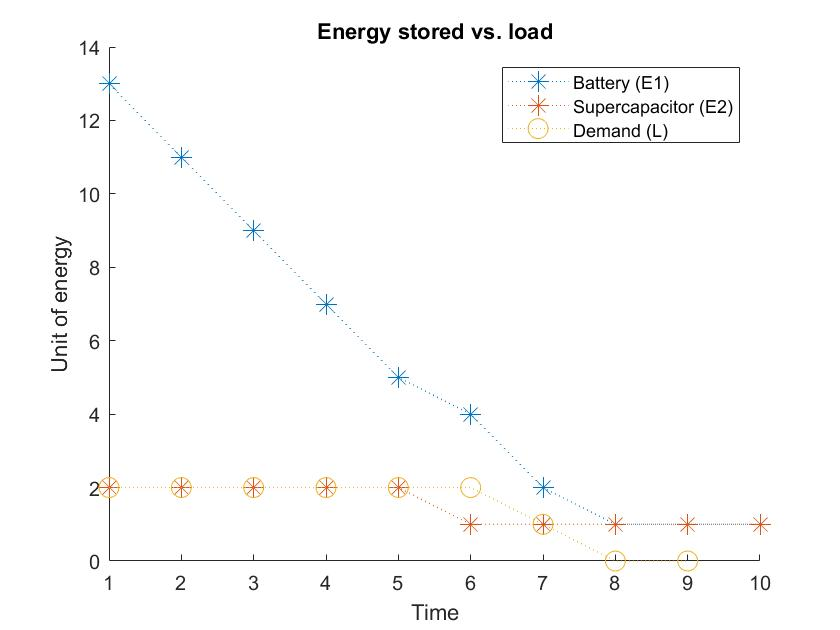
\includegraphics[width=3in,height=1.5in]{EnergyStoredvsload_ConstantLoad(E1_max=13,E2_max=2).jpg}}
\caption{Applying optimal policy from IHDP solution. Constant demand simulation, with N=$14\cdot3=42$, M=16.}
\label{fig}
\end{figure}
\begin{figure}[htbp]
\centerline{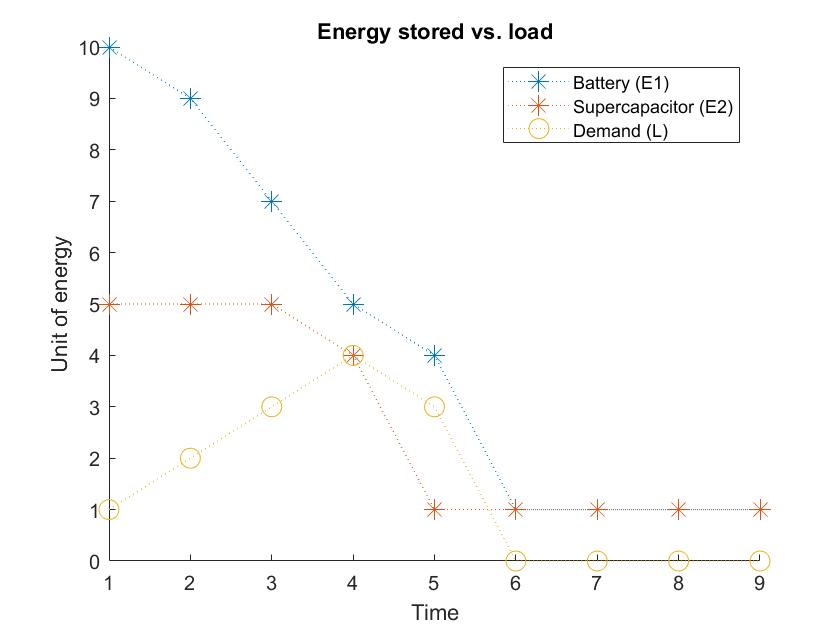
\includegraphics[width=3in,height=1.5in]{EnergyStoredvsload_RampLoad(E1_max=10,E2_max=5).jpg}}
\caption{Applying optimal policy from IHDP solution. Ramp demand simulation, with N=$11\cdot6=66$, M=16.}
\label{fig}
\end{figure} This result is expected because there is low cost for steady use of the battery (constant demand) or for limited cycling (ramp demand).

On the other hand, for fluctuating demand, the supercapacitor is used more, as illustrated in Figure 3.
\begin{figure}[htbp]
\centerline{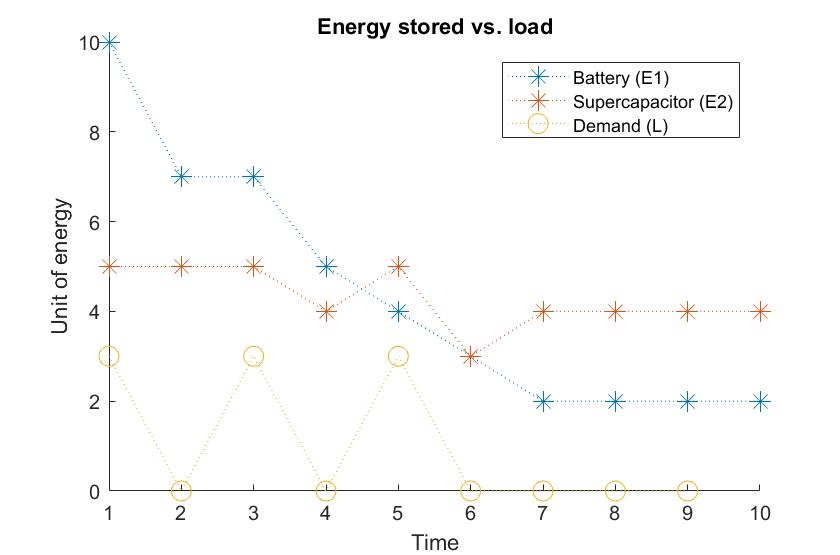
\includegraphics[width=3in,height=1.5in]{EnergyStoredvsFluctuatingLoad(E1=10,E2=5).jpg}}
\caption{Applying optimal policy from IHDP solution. Fluctuating demand simulation, with N=$11\cdot6=66$, M=16.}
\label{fig}
\end{figure} Clearly, the supercapacitor is now discharged at the start. However, this is still not as much use as expected. It was observed that by reducing the discharging efficiency of the battery, the supercapacitor is used more often (see Figure 4).
\begin{figure}[htbp]
\centerline{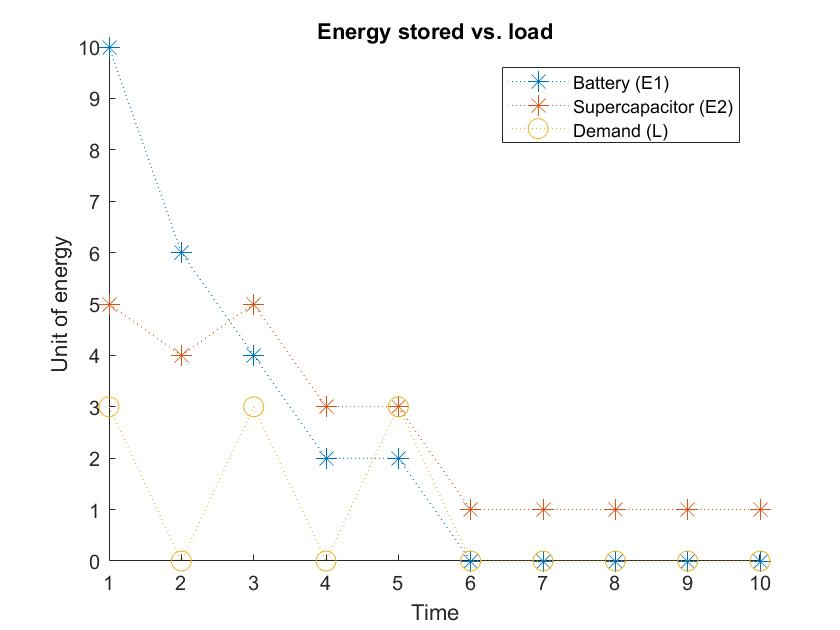
\includegraphics[width=3in,height=1.5in]{EnergyStoredvsFluctuatingLoad_LowBattEff(E1=10,E2=5).jpg}}
\caption{Applying optimal policy from IHDP solution. Fluctuating demand simulation, with N=$11\cdot6=66$, M=16. Lower battery efficiency (50\%).}
\label{fig}
\end{figure} Hence, it is concluded that discharging the battery at the start of the sequence is still preferred because of the higher probability of large initial demands, unless the battery is inefficient.

One should also note how the battery is used to charge the supercapacitor, too. This can be seen, for example, in Figure 3 at time 4, where there is no demand but exchanges in the energy between the storage devices. This also confirms that the optimal policy makes forecasts, since a trade-off is made between instantaneous transfer loss and preempting satisfying future demands from a fully charged supercapacitor. Were it not for the benefits of the latter, there would be no reason for such energy exchanges.

Having characterized the policy obtained from solving the IHDP, the final step in establishing a computationally efficient and equivalent program for this application is to show that the LP gives the same results faster. As explained in Section 6, the policy obtained using LP is the same as long as the primal yields the same optimal solution (costs). Hence, the error in costs obtained using either program needed to be quantified.

In this application, the cost $J(x)$ is a 3-dimensional function of the state $x:=(E_{1},E_{2},L)$, and so would be stored as a 3D matrix for discrete states. A metric for the total error was chosen to be:
\begin{displaymath}
    \frac{\norm{J^{*}_{IHDP}-J_{LP}}_{F}}{\norm{J_{LP}}_{F}}
\end{displaymath} where $\norm{\cdot}_{F}$ denotes the Frobenius norm, $J^{*}_{IHDP}$ is the optimal cost from solving the IHDP, and $J_{LP}$ is the optimal cost from solving the LP. The partially converged cost in IHDP ($J_{IHDP}$) approaches the optimal (converged) cost $J^{*}_{IHDP}$ as the convergence tolerance $\epsilon$ decreases. Hence, if for a given size of state space the error:
\begin{displaymath}
    e_{tot}=\frac{\norm{J^_{IHDP}-J_{LP}}_{F}}{\norm{J_{LP}}_{F}}
\end{displaymath} monotonically decreases as $\epsilon$ decreases, it is known that the LP leads to an equivalent solution as the IHDP. The following table shows results indicating that this is indeed the case:
\begin{table}[htbp]
	\begin{center}
		\begin{tabular}{|c|c|c|}
			\hline
			\textbf{IHDP Convergence Tolerance (\epsilon)}&\textbf{Iterations of IHDP}&\textbf{e_{tot}} \\
			\hline
			1e-3& 5 & 8.24\% \\
			\hline
			1e-4& 12 & 0.423\% \\
			\hline
			1e-6& 1100 & 0.188\% \\
			\hline
		\end{tabular}
		\label{tab1}
	\end{center}
\end{table} Note that this is for a low tolerance in the convergence error of the LP ($\epsilon_{LP}=1e-9$), which is the tolerance on satisfying the constraints of the LP. Hence, it is taken that the LP gives the more accurate solution as $e_{tot}$ decreases to 0.

Finally, in addition to quantifying the error for LP, the LP is also compared to IHDP based on computational complexity. The following table provides simulation results showing that LP generally takes longer to converge for small problems, but is faster for large problems. %While the size of problems and number of cost evaluations were compared in Sections 4 and 5 for the general case, the convergence time is very application-dependent.

\begin{table}[htbp]
	\begin{center}
		\begin{tabular}{|c|c|c|c|}
			\hline
			\textbf{Size of}&\textbf{Tolerances}&\multicolumn{2}{|c|}{\textbf{Number of Iterations}} \\
			\cline{3-4} 
			\textbf{Problem} & & \textbf{IHDP Convergence} &  \textbf{LP Simplex Method} \\
			\hline
			N=30, M=10& 1e-3 & 5 & 15 \\
			\hline
			N=30, M=10& 1e-6 & 12 & 17 \\
			\hline
			N=66, M=16& 1e-3 & 44 & 38 \\
			\hline
			N=66, M=16& 1e-6 & 52 & 47 \\
			\hline
		\end{tabular}
		\label{tab1}
	\end{center}
\end{table}

\section{Conclusion}
In conclusion, this paper has compared the IHDP solution for optimal control to its reformulation as an LP. Theoretical comparison has shown that the LP is likely computationally less expensive. However, practical simulation using the LP formulation is prone to error, and so only an application-specific reduced LP can be compared to IHDP. The results show that optimal control of two storage devices is acheived.

\printbibliography

\end{document}